\chapter{Komplexität und Nicht-Determinismus}
%
In Kapitel~\ref{sec:turingmachine} haben wir formalisiert, was es bedeutet eine Berechnung durchzuführen. Die Turingmaschine ist hierfür unser Werkzeug. Zugleich haben wir in Kapitel~\ref{sec:bigoh} ein relatives Maß zur Beschreibung der Effizienz von Algorithmen eingeführt. Diese Konzepte bilden die Grundlage für die Komplexitätstheorie, welche wir in diesem Kapitel vorstellen wollen.

Im Kapitel~\ref{sec:bigoh} haben wir definiert, dass die $\mathcal{O}$-Notation sowohl auf die Laufzeit als auch andere Ressourcen angewandt werden kann. Wir möchten in diesem Kapitel die $\mathcal{O}$-Notation auf Laufzeit und Speicherverbrauch anwenden.

Wir müssen jetzt unterscheiden beginnen, ob wir eine \emph{deterministische Turingmaschine} (jene Turingmaschine, die wir bisher betrachtet haben) oder eine \emph{nichtdeterministische Turingmaschine} (Turingmaschine, die Nichtdeterminismus unterstützt so wie er auf Seite~\pageref{sec:nondeterminism} beschrieben ist).

\section{Die Klasse \cP{}}
%
Wir möchten nun Klassen für Probleme definieren. Wir definieren die \emph{Klasse \cP{}}:
Das ist jene Klasse, die Probleme umfasst, die auf einer deterministischen Turingmaschine (DTM) in polynomieller Laufzeit gelöst werden können.

Wir haben früher verschiedene Algorithmen betrachtet deren Laufzeit wir asymptotisch analysiert haben. All jene Algorithmen, deren Laufzeit konstant, logarithmisch, linear oder polynomiell mit $n^k$ sind, liegen in der Klasse \cP{}. Dazu zählt Binärsuche oder all jene Algorithmen, die eine fixe Anzahl von verschachtelten Schleifen über die Eingabemenge zur Lösung benötigen.

\section{Die Klasse \cNP{}}
%
Nichtdeterminismus beschreibt die Situation, wenn mehrere Übergänge für eine gegebene Konfiguration existieren. Auf Basis dieses Konzepts definieren wir eine Turingmaschine, welche mehrere Übergänge pro Konfiguration besitzen kann. Dabei wird dieser Turingmaschine eine Orakelturingmaschine zur Verfügung gestellt, welche bei jedem mehrdeutigen Übergang entscheiden kann, welcher von den möglichen Wegen zur korrekten Lösung führt und teilt diese Auswahl unserer nichtdeterministischen Turingmaschine mit.

Für die Klasse \cNP{} gibt es 2 verschiedene Definitionen:
\begin{itemize}
  \item Die Klasse \cNP{} umfasst all jene Probleme, die auf einer nichtdeterministischen Turingmaschine in polynomieller Zeit gelöst werden können.
  \item Gegeben sei eine Lösung für ein Problem. Die Klasse \cNP{} umfasst all jene Probleme für die eine Lösung (ein sogenanntes ,,Zertifikat``) in polynomieller Zeit überprüft (,,verifiziert``) werden kann.
\end{itemize}

\section{Das Erfüllbarkeitsproblem SAT}
%
Elementar für die Betrachtung der Klassen \cP{} und \cNP{} ist das Problem SAT (kurz für englisch ,,Satisfiability``). Dieses stellt die Frage, ob für eine gegebene boolsche Formel (siehe Kapitel~\ref{sec:propositional_logic}) eine erfüllende Belegung gefunden werden kann.

Gegeben sei eine Lösung für SAT (also eine erfüllende Belegung für eine gegebene boolsche Formel). Es ist recht naheliegend, dass die Lösung in polynomieller Zeit verifiziert werden kann. Schließlich ist es dazu nur notwendig alle Operatoren zu evaluieren. Die Anzahl der Operatoren ist nur polynomiell abhängig von der Anzahl der Variablen (was unser $n$ in der $\mathcal{O}$-Notation repräsentieren würde), die in der Formel vorkommen. Daher können wir eine Lösung in polynomieller Zeit verifizieren. Damit ist Definition~2 der Klasse \cNP{} erfüllt.

Für Definition 1 argumentieren wir wie folgt: Wir definieren einen Algorithmus, welcher alle verwendeten Variablen ermittelt (möglich in polynomieller Zeit). Nachfolgend definieren wir nichtdeterministisch eine Zuordnung der Wahrheitswerte zu den Variablen. Diese Zuordnung gibt uns der Algorithmus zurück. Da diese Zuordnung nichtdeterministisch abgelaufen ist, hat uns die Orakelturingmaschine mitgeteilt, welche Zuordnung die Korrekte ist. Auf diese Weise müssen wir nicht alle $2^n$ Variablenbelegungen (sondern nur eine) durchprobieren und erhalten damit einen polynomiellen, nichtdeterministischen Algorithmus.

\section{Reduktionsbeweise}
%
Angenommen wir hätten einen polynomiellen Algorithmus, welcher uns feststellt, ob eine Formel erfüllbar ist. Wir wollen weiters das Problem lösen festzustellen, ob eine Formel nicht erfüllbar ist. In diesem Fall werden wir darauf verzichten einen neuen Algorithmus zu formulieren (sofern er uns keine Vorteile bietet) und den bestehenden Algorithmus wiederverwenden.

Wiederverwendung kann uns helfen Denkarbeit zu sparen. Wir führen noch einen weiteren Gedanken: Wir definierten, dass dieser Algorithmus in polynomieller Zeit Ergebnisse liefert. Die Negation des Ergebnisses ist eine konstante Operation und kann auch durch einen Polynom beschrieben werden. Daraus folgt, dass die gesamte Laufzeit des Algorithmus polynomiell ist. Dem liegt zugrunde, dass die Addition zweier Polynome wieder ein Polynom ist.

Diese Wiederverwendung eines Algorithmus und verarbeiten in einer oberen Zeitschranke wird als ,,Reduktion`` bezeichnet. Wir können das Problem $\overline{\text{SAT}}$ (ob eine boolsche Formel nicht erfüllbar ist) mit einer polynomiellen Reduktion auf SAT (ob eine boolsche Formel erfüllbar its) zurückführen. Wir schreiben:
\[
    \overline{\text{SAT}} \leq_p \text{SAT}
\]

\section{\cNP{}-Vollständigkeit}
%
Unter \cNP{}-Vollständigkeit versteht man eine Eigenschaft von Problemen. \cNP{}-vollständig sind jene Probleme aus
\cNP{}, die polynomiell auf SAT reduziert werden können. Sie sind die ,,schwersten Probleme`` dieser Klasse. Um \cNP{}-Vollständigkeit zu zeigen, müssen folgende Dinge bewiesen werden:
\begin{description}
  \item[membership] Das Problem liegt in \cNP{}.
  \item[hardness] Das Problem kann polynomiell auf SAT reduziert werden.
\end{description}

Interessant ist hierbei, dass es sich um eine transitive Beziehung handelt. Jedes \cNP{}-vollständige Problem kann nicht nur auf SAT, sondern jedes beliebige andere \cNP{}-vollständige Problem reduziert werden. 

Die Klasse der \cNP{}-vollständigen Probleme nennt sich \cNPC{}.
%
\section{\cP{} versus \cNP{}}
%
Die Frage $\mathcal{P} \stackrel{?}{=} \mathcal{NP}$ stellt die wichtigste offene Frage der theoretischen Informatik: Liegen alle Probleme in \cNP{} in \cP{}? Können wir also für jeden Algorithmus auf einer nichtdeterministischen Turingmaschine (welcher polynomielle Zeit benötigt) einen äquivalenten Algorithmus auf einer deterministischen Turingmaschine finden, welcher auch im schlechtesten Fall nur polynomielle Zeit benötigt?

Wir haben festgestellt, dass Probleme aus \cNPC{} die schwersten Probleme von \cNP{} sind. Können wir für einen dieser Probleme einen deterministischen Algorithmus finden, welcher in polynomieller Zeit eine korrekte Lösung findet? Dann fallen die Klassen \cP{} und \cNP{} zusammen, da dann alle ,,einfacheren`` (= nicht-vollständigen) Probleme in \cNP{} auch in polynomieller Zeit gelöst werden können und zwischen allen Problemen in \cNPC{} eine transitive Beziehung besteht.
%
\begin{figure}
  \begin{center}
    \begin{subfigure}[b]{0.4\textwidth}
      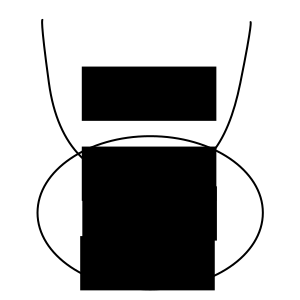
\includegraphics[width=\textwidth]{img/np_neq_p.pdf}
      \caption{wenn \cP{} $\neq$ \cNP{}}
    \end{subfigure}
    \begin{subfigure}[b]{0.4\textwidth}
      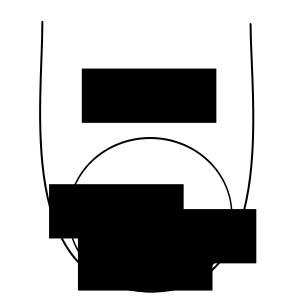
\includegraphics[width=\textwidth]{img/np_eq_p.pdf}
      \caption{wenn \cP{} $=$ \cNP{}}
    \end{subfigure}
  \end{center}
  \caption{Venndiagramm der Klassen \cNP{}, \cP{} und \cNPC{} unter beiden Annahmen}
  \label{fig:p_np_npc}
\end{figure}

In Abbildung~\ref{fig:p_np_npc} ist dargestellt in welcher Beziehung \cP{}, \cNP{} und \cNPC{} zueinander stehen unter der Annahme, dass \cP{} $\subset$ \cNP{} bzw. \cP{} $=$ \cNP{}. \cNP{}-hart sind all jene Probleme, die sich auf SAT reduzieren lassen.

% Turingmaschinen als Basis
% SAT und Hamiltonian Cycle
% P & NP -> P vs NP
